\chapter{Design and Implementation}
\label{chap:design_and_impl}
As a new implementation of SR-Aware NF, we introduce \texttt{End.AN.NF}, which integrates the ability to filter and mangle packets by netfilter into the routing infrastructure in Linux.
\texttt{End.AN.NF} means an \textbf{End} behavior of SR-\textbf{A}ware \textbf{N}ative function for \textbf{N}et\textbf{F}ilter.
We also designed \texttt{End.AN.NF} to leverage the IPv6 routing stack of the Linux kernel. % leverage: 活用する(他動)
An \texttt{End.AN.NF} SID is represented as an IPv6 routing table entry; therefore, its route can be exported and advertised to other nodes via the existing routing protocols and their implementations transparently.
Moreover, \texttt{End.AN.NF} applies netfilter rules to inner packets encapsulated in SRv6.
This enables the use of any netfilter-based applications, such as selective packet discarding and applying NAT for traffic, configured via nftables~\cite{nftables} and iptables~\cite{iptables}, as SR-Aware NFs without modifying their implementations.

netfilter has three hook points in Linux layer-3 packet forwarding flow, which applies netfilter rules to packets at different timings: prerouting, forward, and postrouting.
Figure~\ref{fig:hooks} depicts a flow of transit packets and netfilter hooks to be applied.
As shown, there are two stages for applying netfilter hooks to an SRv6 encapsulated packet as an IPv6 packet including the SRH and its inner packet without the SRH.
First, when a Linux-based SRv6 nodes that implements \texttt{End.AN.NF} receives an IPv6 packet, its kernel applies the prerouting hook to the received packet, and then performs longest prefix matching for the destination IPv6 address as usual.
If the destination address is a local \texttt{End.AN.NF} SID, the kernel passes the packet to the \texttt{End.AN.NF} implementation, otherwise the kernel forwards the IPv6 packet to a corresponding next hop while applying forward and postrouting hooks.
Meanwhile, \texttt{End.AN.NF} applies prerouting, forward, and postrouting hooks again, but to the inner packet encapsulated in the SRH.
During the netfilter applying in the stage of \texttt{End.AN.NF}, the SRH is hidden by \texttt{End.AN.NF}, so netfilter does not have to consider to treat the SRH.%, even if it were a mangle rule.
After \texttt{End.AN.NF} finishes, the destination address of the outer IPv6 header is replaced with the next SID, and the encapsulated packet returns to the usual forwarding path.

\texttt{End.AN.NF} utilizes the \texttt{ARG} field in the SID to mark packets.
\texttt{ARG} is the lower bits of a SID~\cite{rfc8986}.
The SRv6 specification allows End behaviors to utilize \texttt{ARGs} in accordance with their specific behaviors.
In \texttt{End.AN.NF}, \texttt{ARG} of SIDs is attached to packet buffers as a mark.
netfilter-based applications can match the marks on packet buffers and change rules to be applied.
Therefore, operators can adjust rules for traffic based on \texttt{ARG} even behind a single \texttt{End.AN.NF} SID.

Algorithm~\ref{alg:end-an-nf} describes how \texttt{End.AN.NF} passes a packet to a netfilter hook point.
First, \texttt{End.AN.NF} extracts the \texttt{ARG} value from the destination address of a received packet if the \texttt{ARG} length is specified for this \texttt{End.AN.NF} SID.
The extracted \texttt{ARG} value is attached to the packet buffer as a mark.
Next, \texttt{End.AN.NF} switches the head of the packet buffer from the outer SRH to the inner packet, and pass the buffer to a netfilter hook.
After rules installed in the hook are applied to the inner packet, \texttt{End.AN.NF} restores the head of the packet buffer from the inner packet to the outer SRH, and takes the packet to the next process.
This procedure occurs three times for each hook point illustrated as the red rectangles in Figure~\ref{fig:hooks}.

The Linux kernel implements End behaviors as routing table entries whose destinations are SIDs of the functions.
\sloppy This mechanism is called \texttt{seg6local}.
\texttt{End.AN.NF} is one of the End behaviors, so its implementation also leverages \texttt{seg6local}.
As shown in the Figure~\ref{fig:show-route}, we can confirm that the kernel treats the SID representing \texttt{End.AN.NF} as a routing table entry similar to the others End behaviors.
When routing software or iproute2 adds the SID as a routing table entry, it is possible to advertise the routes in the kernel routing table using the traditional routing protocols.
We confirmed that FRRouting~\cite{frr} can advertise SIDs associated with \texttt{End.AN.NF} in the kernel as IPv6 routes to other routers via BGP.
The architecture of \texttt{End.AN.NF} is highly compatible with the existing NFs because it can use the existing routing protocols for routing control.
This architecture is one of the ways to realize SR-Aware NF using Linux netfilter.

\begin{figure}[t]
  \centering
  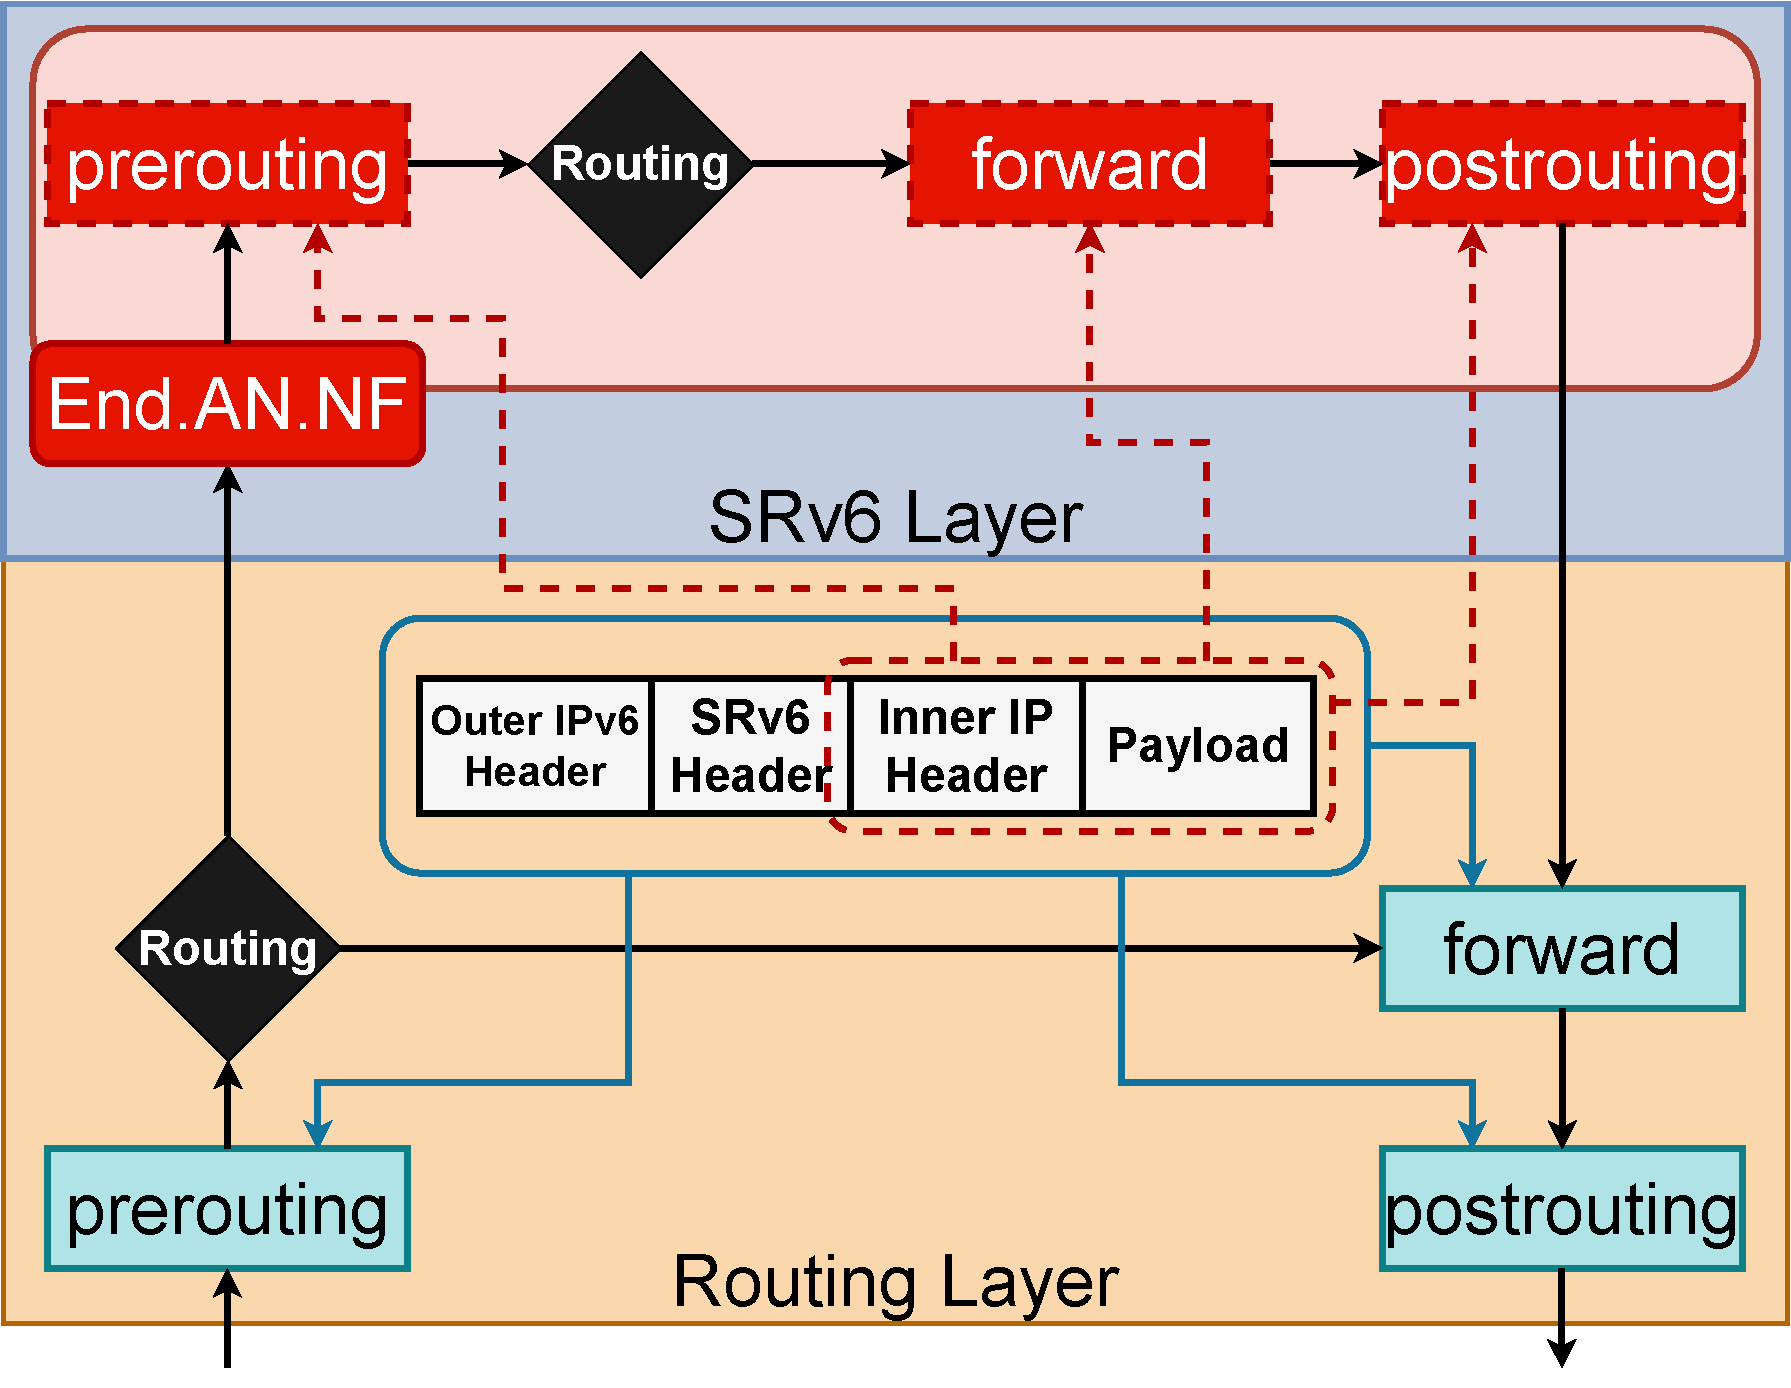
\includegraphics[
    width=0.95\linewidth,
    keepaspectratio=true
  ]{img/End-AN-NF-hooks.pdf}
  \caption{\texttt{End.AN.NF} applies three netfilter hook points, prerouting, forward, and postrouting, to inner packets encapsulated in SRv6.}
  \label{fig:hooks}
\end{figure}

\begin{algorithm*}[t]
  \caption{Pseudo code of passing a packet to a netfilter hook point in \texttt{End.AN.NF}}
  \small
  \label{alg:end-an-nf}
  \begin{algorithmic}[1]
    \if 0
    \Function {Process\_End.AN.NF}{$packet$}
    \State Call function \textbf{Pass\_to\_Hook} with following args: ($packet$, prerouting)
    \State Decrement segleft by 1
    \State Rewrite destination address based on the SID list and segleft, in the SID of the $packet$
    \State Lookup next hop in th routing table entry for rewrite new destination address
    \State Call function \textbf{Pass\_to\_Hook} with following args: ($packet$, forward)
    \State Call function \textbf{Pass\_to\_Hook} with following args: ($packet$, postrouting)
    \EndFunction
    \fi
    % \Function {Pass\_to\_Hook}{$packet$, $hook\_point$}
    \Function {PassPacketToHook}{$packet$}
    \If {the length of $ARG$ is specified for this \texttt{End.AN.NF} SID}
    \State Extract the $ARG$ value from the destination address of outer SRH
    \State Mark the $ARG$ value on the packet buffer $packet$
    \EndIf
    \State Switch the head of packet buffer $packet$ from the outer SRH to the inner packet
    \State Pass $packet$ to a netfilter hook
    \State Switch the head of packet buffer $packet$ from the inner packet to the outer SRH
    \EndFunction
  \end{algorithmic}
\end{algorithm*}

\begin{figure*}[t]
  \centering
  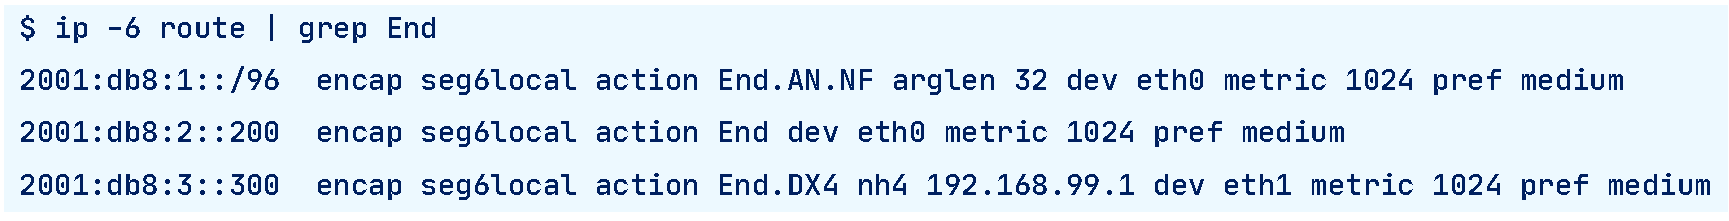
\includegraphics[width=0.95\linewidth]{img/End-FW-show-route.pdf}
  \caption{The modified Linux kernel treats an \texttt{End.AN.NF} SID as an IPv6 routing table entry. We can manage the \texttt{End.AN.NF} routes with the existing tools such as iproute2.}
  \label{fig:show-route}
\end{figure*}